\documentclass[letterpaper]{report}
\usepackage{microtype}
\usepackage{graphicx}
\usepackage{multicol}
\usepackage{url}
\usepackage{changepage}

\title{\kapow{}!\\The Campy Superhero RPG}

\usepackage{enumitem}
\usepackage{pifont}
\usepackage[xcolor]{mdframed}

\newcommand{\kapow}{K\textsc{apow}}

\newcommand{\move}[1]{\textbf{#1}}

\newcommand{\onamiss}{On a miss, be prepared for the worst.}

% The number of arguments to the movedef command
\newcommand{\movedefarity}{3}

\newenvironment{choices}
{\begin{itemize}[label=-,topsep=0cm]\itemsep-0.1cm}
{\end{itemize}}

\newenvironment{chooseone}
{\begin{itemize}[label=\ding{109},topsep=0cm]\itemsep-0.1cm}
  {\end{itemize}}

% Environment for rulebook examples.
\mdfdefinestyle{example}{backgroundcolor=gray!20,hidealllines=true}
\newenvironment{example}
{\begin{mdframed}[style=example]\textbf{\textit{Example: }}}
  {\end{mdframed}}

\newenvironment{example*}
{\begin{mdframed}[style=example]\textbf{\textit{Examples: }}}
{\end{mdframed}}

\begin{document}

\vspace*{\fill}
\thispagestyle{empty}
\begin{centering}
  
\includegraphics[width=3in]{logo}\\
  {\Huge The Campy Superhero Role-Playing Game}\\
  \vspace{1in}
  {\large Rules Version 1.0.0-beta1}\\
\end{centering}
\vspace*{\fill}


\newpage
\thispagestyle{empty}
\vspace*{\fill}

\noindent \copyright 2019 Paul Gestwicki
\vspace{0.5cm}

\noindent Playtesters:
Alex,
Austin Tinkel,
Chris Bucker,
Daniel,
David Mitchell,
Gwyn Hultquist,
Leo,
Nicholas Burrell,
and 
Peter.

\vspace{0.5cm}

\noindent Special thanks to Jessica Gestwicki


\vspace{0.5cm}

\noindent
This work is licensed under a Creative Commons Attribution-NonCommercial-ShareAlike 4.0 International license (CC BY-NC-SA 4.0).\\

\begin{centering}
  % Note: Requires installing texlive-font-utils to automatically convert.
  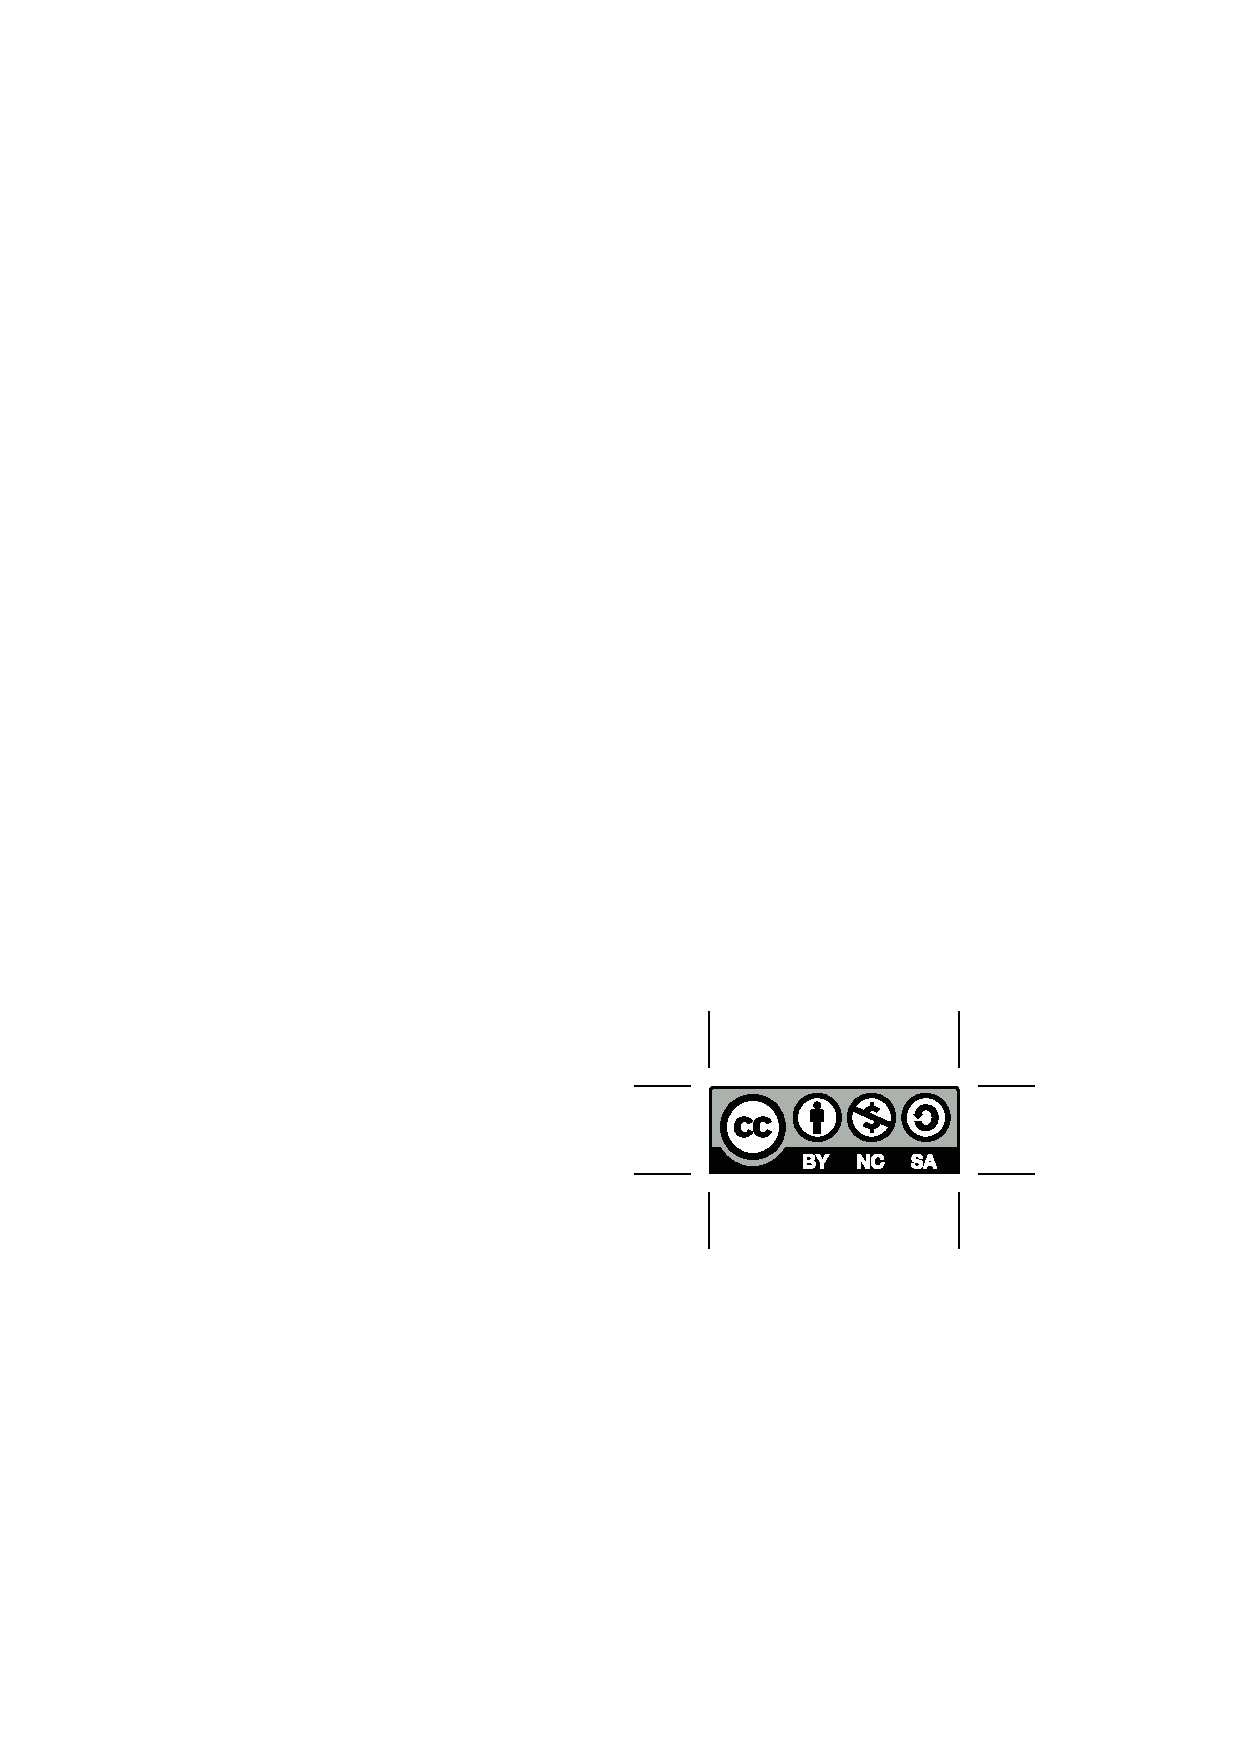
\includegraphics[width=3cm]{by-nc-sa}\\
\end{centering}

\newpage
\pagenumbering{roman}

\tableofcontents{}

\chapter{The Basics}
\pagenumbering{arabic}

\section{Campy Heroics}

Welcome to \kapow{}!

This tabletop role-playing game provides a framework for you
and your friends to create exciting, entertaining, and memorable
stories about a people in tights and masks who fight for justice.

This is a \textit{campy} superhero world, and the rules are designed
to support stories that fall into this genre. The heroes are noble and
honest, and the city doesn't know what they would do without them.
The villains are over-the-top sinister, with schemes that both boggle
and delight the imagination.
When words fail, fists prevail.
Characters use smoke bombs and knock-out gas, not guns and shivs.

The colors are bold and the characters are fundamentally simple.
There are no gritty 1990s anti-heroes, and there are no alternate
universe crossover events.
There are neither mutants nor aliens, and villains with anything you might
call a ``super power'' are extremely rare.
Think 1960s Batman or Johnny Quest, not Superman or the X-Men.

\section{Heroes and Narrators}

The game is designed for a small group of players, ideally no more than six.
All players but one will be \textit{Heroes} who are trying to save
their city from the schemes of hyperbolic villains.
The remaining player will be the \textit{Narrator}, who describes the world
and how it reacts to the heroes' actions.

Since you're reading this book, you're probably going to be the
Narrator. Congratulations! You're going to have a great time. With
just a little genre-appropriate prompting, you should be able to have
your players solving crimes and punching crooks in no time.
More guidance is provided for Narrators later in this book, but first
we have to cover some of the basics.

\subsection*{Playbooks}

Each hero will have a playbook that describes their role on the team.
Every iconic team brings together different characters with
different strengths: Frodo has different talents than Gimli;
Face is sent on missions on which B.\ A.\ Baracus would never succeed;
Batman can get Robin out of trouble, while Robin\ldots{}, well,
he mostly gets in trouble.
The idea behind playbooks will be familiar to those
who have played \textit{Apocalypse World}
or any of its Powered by the Apocalypse progeny.
For those who are new to this style of play but familiar with
some of the industry standard tabletop RPGs, a playbook is like
a character class in \textit{Dungeons \& Dragons} or \textit{Pathfinder}.

\subsection*{Attributes}
A hero has four attributes, which are explained briefly below.
\begin{itemize}
\item \emph{Mighty} is a character's physical prowess--their strength,
  conditioning, and fortitude.
\item \emph{Focused} is a character's control over his mind and body,
  represented in their adroitness, precision, and self-control.
\item \emph{Intellectual} is a character's education and knowledge and their
  ability to apply these to new situations or problems.
\item \emph{Savvy} is a character's ability to operate in and manipulate
  the social world.
\end{itemize}

There are two other important characteristics of the heroes:
Endurance and Experience.
\emph{Endurance} represents how much they can
exert themselves before exhaustion, or how much of a beating they can
take before being critically injured.
Heroes earn \emph{Experience} throughout their adventures
by learning from failure and working together.

\subsection*{Contacts}
Each hero also has a Contact, who is someone outside the hero team
with whom the character has a special bond.
The hero may know the Contact in their heroic identity or in their
secret identity, and the Contact may or may not be aware of the
hero's dual life.
The contact is willing to do favors for the hero, but doing so also tends
to get them into trouble with villains' dastardly plots.

At the start of the game, a hero has a +2 to \move{exhort} their
Contact into action; this is the \textit{reliability} of the contact.
However, as a Narrator move, the reliability may be weakened (see
page~\pageref{move:change-reliability}). If the reliability is ever
reduced to zero, the hero must remove the Contact.

The Narrator is going to want to keep track of the Contacts
so that they can be used during the game. For example, a Contact
provides a great place to bring in a hook~(page~\pageref{sec:hook}).
It is recommended to keep a record of a Contact on an index card,
noting which hero has the Contact, the identities of which the
Contact is aware, and the nature of their relationship, along with
a space for notes you can take during gameplay.

\begin{example}
  Black Mask's Contact is his butler, Alan. During character
  creation, the Narrator makes a card like this:

  \begin{centering}
  \fbox{
    \begin{minipage}[l]{2.5in}
      {\sc Alan} \hfill Black Mask\\
      - Butler\\
      - Aware of secret identity\\     
  \end{minipage}
  }\\
\end{centering}
\end{example}


\subsection*{Bonds}
The relationship your hero has with each other hero is
represented as Bonds. Each hero has a specific Bond rating with
each other hero on the team, measured from -2 to +3. This impacts
how well a hero can help (or hinder!) a teammate.

\section{Moves and Rolls}
Whenever a hero wishes to do something in the world that
is possible and has a chance of failure, they make a \textbf{move}.
Opening an unlocked door does not require a move, but kicking a locked
one open would. Clapping your hands does not require a move, but
wriggling free when your hands are tied does.

To make a move, you choose the appropriate move from the basic moves
list or your playbook, then you roll two six-sided dice and add them
together, along with any relevant modifiers.  Generally speaking, a
result of 10+ means it is an unmitigated success. A total of 7--9
means that success comes at a cost. A total of 6 or lower means that
you have failed and the Narrator will be able to respond with a move
of their own (see Narrator Moves on page~\pageref{sec:narrator-moves}).

The basic moves that are available to every hero are named below,
and their full definitions can be found on page~\pageref{sec:basic-moves}.
\newenvironment{movedef}[\movedefarity]
{\item #1}{}
\begin{itemize}
  \setlength\itemsep{0px}
  \begin{movedef}{Rumble}
{
  When you \move{rumble}, you and your opponent each lose one Endurance,
  but first roll+Mighty. On a 10+, choose two. On a 7--9, choose one.
  \begin{choices}
    \item Remove one additional Endurance from your opponent.
    \item Wrest an item from an enemy or force it to be dropped.
    \item Put up a good defense and prevent one Endurance loss.
    \item Frighten your opponent.
    \end{choices}
  Gain +1 if you \emph{use the environment}.  
  \onamiss{}
}
{
  Every good episode includes at least one tussle between the heroes
  and some stooges, and this move provides the framework for it.
  The move encapsulates a range of actions that might come up
  in a campy rumble, including breaking vases over someone's head,
  delivering a swinging kick from a chandelier,
  sword-fighting with weapons taken from a museum case,
  and of course, good old-fashioned fisticuffs.

  A Villain's lackeys share a pool of Endurance, so each point
  of Endurance damage done to them removes one of them from
  the battle.
  If a hero chooses to frighten an opponent during the rumble,
  that opponent must do their best to change their current course
  of action.
  
  The Narrator should set up a fun and iconic environment in which a rumble
  can take place. When a player declares their move, if they
  \emph{use the environment} in a way
  that no other player has yet used, they get a +1 to the roll.

  \begin{example}
    The Black Mask has the drop on some goons. The player declares, ``I will swing in on my Black Mask Rope and deliver a solid kick!''

    The Narrator responds, ``Yeah, take a +1!'' The Black Mask rolls
    a total of 11 and chooses to prevent his own Endurance loss
    and to remove an additional Endurance from the opponent.
  \end{example}


  \begin{example}
    The Black Mask is surrounded by three ruffians. He gets into the
    rumble, rolling a 7, and chooses to frighten an opponent.
    The Narrator tells him that as he slugs one of the ruffians,
    another one backs away, saying, ``This ain't worth it!'' and
    leaves the scene.
  \end{example}
}
\end{movedef}

\begin{movedef}{Heroic Feat}
{
  When you \move{attempt a heroic feat}, roll+Mighty. On a 10+, you are
  successful. On a 7--9, you are successful and choose one.
  \begin{choices}
  \item An ally or civilian is placed in immediate danger.
  \item There is an unintended side-effect.
  \item You lose one Endurance.
  \end{choices}
  \onamiss{}
}
{
  Sometimes a hero is called upon to do some heroic physical feat,
  such as throwing a rock to knock over a bottle across the room,
  holding a mechanical door open while the orphans escape the fire,
  or leaping across a gap between buildings.
  When other moves don't cut it, make a heroic feat.

  Note that the heroic feat should never replace any of the
  playbook moves. For example, you cannot use a Heroic
  Feat to slip silently out of the ropes binding your hands
  behind your back: that's the Daredevil's \move{escape bonds}
  move. 
}
\end{movedef}

\begin{movedef}{Prowl}
  {
    When you \move{prowl}, roll+Focused. On a 10+, you are undetected and take +2 forward. On a 7--9, choose one of the following.
    \begin{choices}
    \item You are undetected but are hindered; take -2 forward.
    \item You must choose between being detected or a negative consequence.
    \end{choices}
    \onamiss{}    
  }
  {
    This move allows heroes to sneak, to spy, or to lurk without being
    detected. It is often used to try to get the drop on a group
    of foes who are in an otherwise well-defended position.
    
    \begin{example}
      Black Mask decides to sneak his way into the warehouse to get
      the drop on the goons. He rolls an 8 and opts to take the choice.
      The Narrator explains, ``As you drop in through the open window,
      you see one of the goons about to pour the mind-control serum
      onto the candy bars. Do you reveal yourself to stop them
      from doing this, or do you stay in the shadows, undetected?''
    \end{example}
  }
\end{movedef}

\begin{movedef}{Race / Chase}
  {
    When you \move{race against the clock} to a target or \move{chase}
    a target, roll+Focused. On
    a 10+, you reach your target. On a 7--9, you reach your target and
    must choose one of the following.
    \begin{choices}
    \item You or an ally are placed in grave danger.
    \item You lose one Endurance.
    \end{choices}
    \onamiss{}
  }
  {
    This move comes up when the heroes are chasing down villains
    or trying to get to the bank before the bomb goes off.
    It is agnostic of the mode of transportation: from a narrative
    point of view, the pursuit is what matters, not whether it is
    in a car, in a boat, or on foot. The implication there comes in
    how the Narrator might respond to failure.

    \begin{example}
      Black Mask knocks out the last of the flunkies and turns
      around to see The Paradox fleeing the scene on foot.
      Black Mask decides to chase, and his total roll is 10:
      Black Mask grabs The Paradox and holds him until the
      police arrive to take him away.
    \end{example}

    \begin{example}
      Naturally, The Paradox has escaped from prison and kidnapped
      the mayor's daughter. Black Mask knows that The Paradox will
      sail away from the marina to his island hideout
      any moment, so he hops into the Black\-Mask\-Mo\-bile
      and races across town.
      He rolls a 5, arriving on the coast just in time to see
      The Paradox's ship moving over the horizon.
      Black Mask will have to find another way to save the
      innocent civilian.
    \end{example}
  }
\end{movedef}

\begin{movedef}{Investigate}
  {
    \label{move:investigate}
    When you \move{investigate a scene},
    roll+Intellectual. On a 10+, either \emph{ask} two of the
    following or
    \emph{deduce} a true answer to one.  On a 7--9,
    ask one of the following. The Narrator's answers will be true.    
    \begin{choices}
    \item Who was behind this?
    \item What happened here?
    \item What was the purpose of this?
    \item Who is endangered by this?
    \item What is significant here?
    \item What is my biggest threat right now?
    \item What is the best way in / out / through?
    \end{choices}
    \onamiss{}
  }
  {
    This move is used whenever a hero is trying to find clues in 
    a location or situation. The pace is up to the situation:
    an investigation may be an hour at a crime scene or it may
    be a glance around a room during a brawl.

    A player who investigates successfully has to make an important
    choice to either \emph{ask} a question about the world
    or to \emph{deduce} a truth about the world.
    When asking, the Narrator will provide answers that are true.
    Note that the Narrator does not need to extrapolate on the
    answers: asking who is behind a crime, for example, will reveal
    a name but not a motive.
    If the player chooses to deduce an answer, then they make a
    true statement about the world. Only the specific answer to the
    question is binding to the narrative, not any additional
    extrapolation.

    A player making this move may simply ask a question that is on
    their minds rather than one from the list. In this case,
    a Narrator can answer the closest question to what was asked.

    \begin{example}
      Black Mask arrives at the scene of the kidnapping and decides
      to \move{investigate}. He rolls an 11 and decides to ask
      what happened and who was behind it.
      The Narrator explains, ``You find an eyewitness who tells you
      that the culprit was wearing a garish black-and-white suit.
      He hypnotized the victim, who then entered willingly into
      a black-and-white striped van. This sounds like the work
      of The Paradox!''
    \end{example}

    \begin{example}
      The Fly is on the scene of a bank robbery and decides to
      \move{investigate}, rolling a perfect 12.
      She decides to deduce the truth of who was behind
      this, saying, ``There's only
      one Villain bold enough to rob a bank during broad daylight,
      knowing it would draw me to the scene of the crime.
      It must be my old arch-nemesis, DDT!''
    \end{example}
  }
\end{movedef}

\begin{movedef}{Scrutinize}
  {
  When you \move{scrutinize a person},  roll+Savvy. On a 10+, hold 3. On a 7--9, hold 1. While you are interacting with the target and nothing externally significant changes, spend a hold to ask one of the following.
  \begin{choices}
    \item Are they telling the truth?
    \item What are they feeling?
    \item What is their intent?
    \item What do they wish I would do?
    \end{choices}
    On a miss, hold 1 anyway and be prepared for the worst.
  }
  {
    When a hero is not sure if an NPC is being straight with them or not,
    it's a good time to scrutinize them. The hero draws upon their
    wit, charm, and worldliness to divine the truth.

    \begin{example}
      Black Mask is asking the security guard what happened
      at the museum and decides to \move{scrutinize} him.
      He rolls an 8 and marks a hold of 1. Black Mask asks,
      ``How did the criminals get into the museum?''
      The security guard responds that they must have picked the lock
      on the door, but this sounds fishy: Black Mask spends his
      hold to ask if he is telling the truth.
      The Narrator tells Black Mask that they could not have
      picked the lock: the security guard is hiding something.
    \end{example}
  }
\end{movedef}

\begin{movedef}{Exhort}
{
  When you \move{exhort an NPC to do something}, tell them what
  you want and give them a reason, then roll+Savvy. On a 10+, they
  go along with you until or unless the reason is betrayed. On a
  7--9, they will go along with you if given concrete assurance,
  collaboration, or evidence. \onamiss{}
}
{
  This move is for those times that a hero needs an NPC to do something
  they would not do otherwise. The hero needs to have some kind of
  leverage over the NPC, even if it is simply appealing to their sense
  of justice and honor (which, of course, only works on an NPC who
  has such sensibility).
 
  If a hero fails to exhort a Contact into action, the Narrator should
  seriously consider reducing the reliability of the Contact.  Even
  just doing this one can help the heroes understand that their
  Contacts are trusted allies and not tools to abuse.

  \begin{example}
    The police have already arrived at the scene of the burglary and
    have been instructed not to let anyone into the area.
    The Fly \move{exhorts} them to let her investigate the scene.
    She rolls a 9, and so she gives them assurance that she
    is working on behalf of the commissioner. This satisfies the
    police, who are aware of her stellar reputation.
  \end{example}
}
\end{movedef}

\begin{movedef}{Help or Hinder}
  {
    When you \move{help} or \move{hinder} another hero, roll+bond. On a 10+, give a +2 or -2 to their roll. On a 7--9, give a +1 or -1 to their roll. \onamiss{}
  }
  {
    A hero in a position to help an ally can do so with this move.
    Before the other hero makes a move of their own, the helping hero
    explains how they can assist, and then makes this move.
    Multiple heroes may attempt to help, but only the highest bonus
    contributes, while every failure still counts.
    
    In rare cases, a hero may wish to hinder another hero from an action.
    This works the same way as helping, except that the bonuses become
    penalties.

    \begin{example}
      Black Mask grabs his dice declares his intent to \move{rumble} with the
      villains in the department store.
      The Fly shouts, ``Hang on, I'll throw you a mannequin you can use
      to bash them around.'' This constitutes \move{help} with the Black
      Mask, so The Fly rolls, adding her Bond with her teammate,
      and gets a 10. Black Mask catches the mannequin and quips
      about making a swing at the real dummies as he gets a +2 to
      his \move{rumble} move.
    \end{example}
  }
\end{movedef}

\end{itemize}

Failing a roll may put the heroes in a bad situation, but heroes
can learn from their failures.
Each time your hero misses a roll, mark one Experience.

\begin{example}
  Black Mask is in a tussle with a group of lackeys.
  He rolls a 4, so even with his +1 Might, he fails the roll.
  The Narrator tells him that the lackeys overwhelm him,
  pinning him to the wall. The Black Mask learns something
  that day about fighting too many enemies at once, and
  he marks one Experience. Meanwhile, the Narrator chooses
  a move of their own.
\end{example}

Some moves give players a bonus or penalty \emph{forward}.
This means that on their next move, they apply that given bonus
or penalty in full. After the bonus or penalty is applied to a roll,
it is dismissed; the player no has zero \emph{forward}.

\begin{example}
  Black Mask and Captain Amazing are eyeing down
  the brutish bodyguards of the Barracuda.
  Captain Amazing gives an inspiring speech that grants
  The Black Mask +2 forward.
  Black Mask charges into the battle, adding an extra +2 to
  his rumble move. After mopping the floor with the bodyguards,
  Black Mask decides to investigate the scene. He already
  used his +2 forward, so there are no other special modifiers
  to his investigation.
\end{example}

Finally, some moves, such as \move{scrutinize}, give a hero \emph{hold}.
This means that the player marks a number of hold on their character
sheet and can spend them later for the indicated effect.
A player can only have \emph{hold} for one purpose at a time:
if they make a new move that grants \emph{hold}, the previous is lost.

\section{The First Session}

Before the First Session, the Narrator needs to do a little
preparation: creating a Villain and a short Scheme
that the heroes can try to unravel.
See page~\pageref{sec:session-prep} for additional notes
on how to create Villains and Schemes.
Make sure you have printed out copies of the playbooks and the moves
handouts, all of which can be found on the \kapow{} project Web site.

The first time you and your friends sit down to play the game,
you are going to need to create some characters and the ties
that bind them together.
\kapow{} is designed to make character creation fast, fun,
and interactive.

It's a good idea for the Narrator to start by reminding the players
about the campy superhero genre.
After that, they might explain the fundamental systems of the game:
players roll dice to make moves, and rolls are given bonuses
based on their character's attributes. 

The first step to making characters is to establish some
properties of their team.
Place the Team handout in the middle of the table and follow
the instructions from there.
Throughout the team and hero creation process,
cases where players must commit to a choice
are presented as open circles (\ding{109}) that
can be filled in or checked.

When it gets time to choose playbooks, the Narrator can read off
the short introductory blurb for each.
Each player selects a playbook for their hero. Two players may not
choose the same playbook.
The playbook then walks players through the hero creation process.

Once all the players are in the \emph{Bonds} step, then they go around
the table introducing themselves.
As a player shares the name of their hero, each other player should
write down the hero's name on their own sheets in order to
track their Bond with that hero.
Players should 
mention their character's heroic and secret identities, even if their selected
background means that their secrets are not known to the other
players. This can be considered ``off camera'' knowledge that the
players have but their characters do not.
Then, the players go around the table again, this time asking
any optional questions in the \emph{Bonds} section and then documenting
their initial Bonds.
Once Bonds are established, the players return to the Team sheet
for the final team creation steps.

Now that the characters have been created and introduced to each other,
it's time to get into the adventure.
The Narrator should give the hook for the adventure and then ask the
players, ``What do you do?''


\chapter{Hero Rules}

As a hero in the game, each interaction you have with the world
will be a \emph{move}. The general principle of playing \kapow{} is
``to do it, do it.''
That is, if you want your character to take action, identify the
most appropriate move, state it, and roll those dice.
If you are a new player, the Narrator may help you turn your
intention into moves, but this will become natural to you
in short order.

This chapter includes the definitions for all the \emph{basic moves}
to which all heroes have access. Heroes also have playbook-specific
moves that they may have selected during character creation or
advancement.  There are also a few \emph{special moves} that come up
in particular situations rather than in response to your intention.
The end of the chapter includes rules for dealing with
Endurance recovery and injury as well as optional rules for very young
players.

\renewenvironment{movedef}[\movedefarity]
{\subsection*{#1}
  \begin{adjustwidth}{0.25in}{0.25in}
    {\itshape #2}\vspace{0.2cm}
  \end{adjustwidth}

  #3}
{}

\section{Basic Moves}
\label{sec:basic-moves}

Below are the moves to which all heroes have access, regardless
of their playbooks. Like their playbook moves, players can invoke
them at any time that they are appropriate during a session.

\begin{movedef}{Rumble}
{
  When you \move{rumble}, you and your opponent each lose one Endurance,
  but first roll+Mighty. On a 10+, choose two. On a 7--9, choose one.
  \begin{choices}
    \item Remove one additional Endurance from your opponent.
    \item Wrest an item from an enemy or force it to be dropped.
    \item Put up a good defense and prevent one Endurance loss.
    \item Frighten your opponent.
    \end{choices}
  Gain +1 if you \emph{use the environment}.  
  \onamiss{}
}
{
  Every good episode includes at least one tussle between the heroes
  and some stooges, and this move provides the framework for it.
  The move encapsulates a range of actions that might come up
  in a campy rumble, including breaking vases over someone's head,
  delivering a swinging kick from a chandelier,
  sword-fighting with weapons taken from a museum case,
  and of course, good old-fashioned fisticuffs.

  A Villain's lackeys share a pool of Endurance, so each point
  of Endurance damage done to them removes one of them from
  the battle.
  If a hero chooses to frighten an opponent during the rumble,
  that opponent must do their best to change their current course
  of action.
  
  The Narrator should set up a fun and iconic environment in which a rumble
  can take place. When a player declares their move, if they
  \emph{use the environment} in a way
  that no other player has yet used, they get a +1 to the roll.

  \begin{example}
    The Black Mask has the drop on some goons. The player declares, ``I will swing in on my Black Mask Rope and deliver a solid kick!''

    The Narrator responds, ``Yeah, take a +1!'' The Black Mask rolls
    a total of 11 and chooses to prevent his own Endurance loss
    and to remove an additional Endurance from the opponent.
  \end{example}


  \begin{example}
    The Black Mask is surrounded by three ruffians. He gets into the
    rumble, rolling a 7, and chooses to frighten an opponent.
    The Narrator tells him that as he slugs one of the ruffians,
    another one backs away, saying, ``This ain't worth it!'' and
    leaves the scene.
  \end{example}
}
\end{movedef}

\begin{movedef}{Heroic Feat}
{
  When you \move{attempt a heroic feat}, roll+Mighty. On a 10+, you are
  successful. On a 7--9, you are successful and choose one.
  \begin{choices}
  \item An ally or civilian is placed in immediate danger.
  \item There is an unintended side-effect.
  \item You lose one Endurance.
  \end{choices}
  \onamiss{}
}
{
  Sometimes a hero is called upon to do some heroic physical feat,
  such as throwing a rock to knock over a bottle across the room,
  holding a mechanical door open while the orphans escape the fire,
  or leaping across a gap between buildings.
  When other moves don't cut it, make a heroic feat.

  Note that the heroic feat should never replace any of the
  playbook moves. For example, you cannot use a Heroic
  Feat to slip silently out of the ropes binding your hands
  behind your back: that's the Daredevil's \move{escape bonds}
  move. 
}
\end{movedef}

\begin{movedef}{Prowl}
  {
    When you \move{prowl}, roll+Focused. On a 10+, you are undetected and take +2 forward. On a 7--9, choose one of the following.
    \begin{choices}
    \item You are undetected but are hindered; take -2 forward.
    \item You must choose between being detected or a negative consequence.
    \end{choices}
    \onamiss{}    
  }
  {
    This move allows heroes to sneak, to spy, or to lurk without being
    detected. It is often used to try to get the drop on a group
    of foes who are in an otherwise well-defended position.
    
    \begin{example}
      Black Mask decides to sneak his way into the warehouse to get
      the drop on the goons. He rolls an 8 and opts to take the choice.
      The Narrator explains, ``As you drop in through the open window,
      you see one of the goons about to pour the mind-control serum
      onto the candy bars. Do you reveal yourself to stop them
      from doing this, or do you stay in the shadows, undetected?''
    \end{example}
  }
\end{movedef}

\begin{movedef}{Race / Chase}
  {
    When you \move{race against the clock} to a target or \move{chase}
    a target, roll+Focused. On
    a 10+, you reach your target. On a 7--9, you reach your target and
    must choose one of the following.
    \begin{choices}
    \item You or an ally are placed in grave danger.
    \item You lose one Endurance.
    \end{choices}
    \onamiss{}
  }
  {
    This move comes up when the heroes are chasing down villains
    or trying to get to the bank before the bomb goes off.
    It is agnostic of the mode of transportation: from a narrative
    point of view, the pursuit is what matters, not whether it is
    in a car, in a boat, or on foot. The implication there comes in
    how the Narrator might respond to failure.

    \begin{example}
      Black Mask knocks out the last of the flunkies and turns
      around to see The Paradox fleeing the scene on foot.
      Black Mask decides to chase, and his total roll is 10:
      Black Mask grabs The Paradox and holds him until the
      police arrive to take him away.
    \end{example}

    \begin{example}
      Naturally, The Paradox has escaped from prison and kidnapped
      the mayor's daughter. Black Mask knows that The Paradox will
      sail away from the marina to his island hideout
      any moment, so he hops into the Black\-Mask\-Mo\-bile
      and races across town.
      He rolls a 5, arriving on the coast just in time to see
      The Paradox's ship moving over the horizon.
      Black Mask will have to find another way to save the
      innocent civilian.
    \end{example}
  }
\end{movedef}

\begin{movedef}{Investigate}
  {
    \label{move:investigate}
    When you \move{investigate a scene},
    roll+Intellectual. On a 10+, either \emph{ask} two of the
    following or
    \emph{deduce} a true answer to one.  On a 7--9,
    ask one of the following. The Narrator's answers will be true.    
    \begin{choices}
    \item Who was behind this?
    \item What happened here?
    \item What was the purpose of this?
    \item Who is endangered by this?
    \item What is significant here?
    \item What is my biggest threat right now?
    \item What is the best way in / out / through?
    \end{choices}
    \onamiss{}
  }
  {
    This move is used whenever a hero is trying to find clues in 
    a location or situation. The pace is up to the situation:
    an investigation may be an hour at a crime scene or it may
    be a glance around a room during a brawl.

    A player who investigates successfully has to make an important
    choice to either \emph{ask} a question about the world
    or to \emph{deduce} a truth about the world.
    When asking, the Narrator will provide answers that are true.
    Note that the Narrator does not need to extrapolate on the
    answers: asking who is behind a crime, for example, will reveal
    a name but not a motive.
    If the player chooses to deduce an answer, then they make a
    true statement about the world. Only the specific answer to the
    question is binding to the narrative, not any additional
    extrapolation.

    A player making this move may simply ask a question that is on
    their minds rather than one from the list. In this case,
    a Narrator can answer the closest question to what was asked.

    \begin{example}
      Black Mask arrives at the scene of the kidnapping and decides
      to \move{investigate}. He rolls an 11 and decides to ask
      what happened and who was behind it.
      The Narrator explains, ``You find an eyewitness who tells you
      that the culprit was wearing a garish black-and-white suit.
      He hypnotized the victim, who then entered willingly into
      a black-and-white striped van. This sounds like the work
      of The Paradox!''
    \end{example}

    \begin{example}
      The Fly is on the scene of a bank robbery and decides to
      \move{investigate}, rolling a perfect 12.
      She decides to deduce the truth of who was behind
      this, saying, ``There's only
      one Villain bold enough to rob a bank during broad daylight,
      knowing it would draw me to the scene of the crime.
      It must be my old arch-nemesis, DDT!''
    \end{example}
  }
\end{movedef}

\begin{movedef}{Scrutinize}
  {
  When you \move{scrutinize a person},  roll+Savvy. On a 10+, hold 3. On a 7--9, hold 1. While you are interacting with the target and nothing externally significant changes, spend a hold to ask one of the following.
  \begin{choices}
    \item Are they telling the truth?
    \item What are they feeling?
    \item What is their intent?
    \item What do they wish I would do?
    \end{choices}
    On a miss, hold 1 anyway and be prepared for the worst.
  }
  {
    When a hero is not sure if an NPC is being straight with them or not,
    it's a good time to scrutinize them. The hero draws upon their
    wit, charm, and worldliness to divine the truth.

    \begin{example}
      Black Mask is asking the security guard what happened
      at the museum and decides to \move{scrutinize} him.
      He rolls an 8 and marks a hold of 1. Black Mask asks,
      ``How did the criminals get into the museum?''
      The security guard responds that they must have picked the lock
      on the door, but this sounds fishy: Black Mask spends his
      hold to ask if he is telling the truth.
      The Narrator tells Black Mask that they could not have
      picked the lock: the security guard is hiding something.
    \end{example}
  }
\end{movedef}

\begin{movedef}{Exhort}
{
  When you \move{exhort an NPC to do something}, tell them what
  you want and give them a reason, then roll+Savvy. On a 10+, they
  go along with you until or unless the reason is betrayed. On a
  7--9, they will go along with you if given concrete assurance,
  collaboration, or evidence. \onamiss{}
}
{
  This move is for those times that a hero needs an NPC to do something
  they would not do otherwise. The hero needs to have some kind of
  leverage over the NPC, even if it is simply appealing to their sense
  of justice and honor (which, of course, only works on an NPC who
  has such sensibility).
 
  If a hero fails to exhort a Contact into action, the Narrator should
  seriously consider reducing the reliability of the Contact.  Even
  just doing this one can help the heroes understand that their
  Contacts are trusted allies and not tools to abuse.

  \begin{example}
    The police have already arrived at the scene of the burglary and
    have been instructed not to let anyone into the area.
    The Fly \move{exhorts} them to let her investigate the scene.
    She rolls a 9, and so she gives them assurance that she
    is working on behalf of the commissioner. This satisfies the
    police, who are aware of her stellar reputation.
  \end{example}
}
\end{movedef}

\begin{movedef}{Help or Hinder}
  {
    When you \move{help} or \move{hinder} another hero, roll+bond. On a 10+, give a +2 or -2 to their roll. On a 7--9, give a +1 or -1 to their roll. \onamiss{}
  }
  {
    A hero in a position to help an ally can do so with this move.
    Before the other hero makes a move of their own, the helping hero
    explains how they can assist, and then makes this move.
    Multiple heroes may attempt to help, but only the highest bonus
    contributes, while every failure still counts.
    
    In rare cases, a hero may wish to hinder another hero from an action.
    This works the same way as helping, except that the bonuses become
    penalties.

    \begin{example}
      Black Mask grabs his dice declares his intent to \move{rumble} with the
      villains in the department store.
      The Fly shouts, ``Hang on, I'll throw you a mannequin you can use
      to bash them around.'' This constitutes \move{help} with the Black
      Mask, so The Fly rolls, adding her Bond with her teammate,
      and gets a 10. Black Mask catches the mannequin and quips
      about making a swing at the real dummies as he gets a +2 to
      his \move{rumble} move.
    \end{example}
  }
\end{movedef}


\section{Special Moves}

The following special moves only come up in particular circumstances.
Players generally do not have agency over when they arise,
but neither are they Narrator moves that are played in response
to heroes' failures.

\begin{movedef}{Take a hit}
{
  When you \move{take a hit}, you roll+endurance lost. On a 10+, the
  Narrator chooses one.
  \begin{choices}
  \item You are hit in a vulnerable spot. Lose an extra point of Endurance.
  \item You are incapacitated (for example, unconscious, hypnotized, or panicked).
  \end{choices}
  On a 7--9, the Narrator chooses one.
  \begin{choices}
  \item You drop what you are holding.
  \item You lose your footing.
  \item You lose track of something or someone important to the scene.
  \end{choices}
  On a miss, the Narrator may choose one of the 7--9 list above,
  but this is instead of one point of the Endurance loss that
  instigated this move.
}
{
  This is an optional move that the Narrator can call for
  when a hero takes a hit outside of a rumble.
  It is primarily used in conjunction with the \move{reduce their
    Endurance} narrator move (see page~\pageref{move:reduce-endurance}).
  ``Taking a hit'' is a general term for any kind of physical
  injury, such as falling from a great height, being struck by
  a vehicle, choking on the gas from a smoke grenade,
  or any of the other sorts of physical peril that heroes tend
  to find themselves in.
}
\end{movedef}

\begin{movedef}{End of session}
{
  \move{At the end of every session}, choose one character
  whom you trust more than before. Tell that player to add +1
  to their Bond with you. If this brings them to Bond~+4, they reset
  to Bond~+1 and mark Experience. If you do not trust any of your
  teammates more than before, than chose one character in whom you
  had hoped to gain trust but did not. Tell that player to add -1 to
  their Bond with you. If this brings them to Bond~-3, they reset to
  Bond~0 and they Mark experience.
}
{
  This move is made at the end of a session, whether it's the
  conclusion of a story or a cliffhanger.
  It serves two purposes. Mechanically, it represents the changing
  relationships among heroes. Narratively, it provides an opportunity
  to recap some of the most important moments of the session.
}
\end{movedef}

\section{Endurance and Rest}

Each character has limited Endurance. Endurance is lost by being
injured, such as in a brawl, by inhaling poisonous gas, or when
falling off a rooftop. When a character loses Endurance, their
player marks off a box on the Endurance tracker.
Marking off an Endurance box with a ``-1'' means that the hero takes
-1 to all rolls, independent of other bonuses or penalties.
The character is said to be \emph{imperiled}.

At the end of a scene, a character who is not imperiled may recover
Endurance, at the Narrator's discretion. Essentially, if there is any
time to catch your breath, you recover Endurance. A character who
became imperiled recovers to just beyond peril threshold.

A character who must lose Endurance and has no more spaces on the
Endurance tracker is in \emph{critical condition}. The player chooses one of
the following.
\begin{choices}
\item The character recovers Endurance at the Narrator's discretion but
  suffers a permanent -1 to Mighty. 
\item The character suffers a wound or trauma that permanently
  bans them from heroic life, and the character becomes
  an NPC.
\item The character dies.
\end{choices}
If the character survives critical condition, the Narrator can
determine how much Endurance is granted the character.

\section{Sidekicks}

Optionally, you can play \kapow{} with children who may not have the
reading ability or patience to deal with moves and playbooks.
These are called \emph{sidekicks}.
Odds are that if you're playing with a sidekick, you know the kid
and know they can handle.  The main idea here is that
you can incorporate such players to the extent they will enjoy it, and
it fits well in the genre.

An easy way to create a sidekick is to have the player draw their
character, and then you can ask them about it. Help them come up
with a name that fits the genre, and that's about all you need.
If they understand the idea of secret identities, you could have
them also draw what the character looks like when not in costume.

The rest of the team tracks their Bond with the sidekick, just like
the other heroes. However, the sidekick does not need to bother with
the bookkeeping of Bonds.

Sidekicks don't need attributes, nor do they track Endurance.
Rather, when they want to take an action that fits the normal
rules for a move---that is, it fits the narrative and
there's a reasonable chance of success or failure---have them
roll two six-sided dice and add them together.
On a roll of 7+, they succeed; otherwise, they fail.
The Narrator may choose to take a move in response to the failure,
but if they do, it should be something ``soft'' such as foreshadowing
future trouble.

\chapter{Narrator Rules}

This chapter contains all the rules for the Narrator.
As mentioned earlier, the Narrator needs to be familiar with all
the rules in the game in order to keep a good flow.
However, keep in mind one of the cardinal rules of tabletop
role-playing: it's almost always better to rule on the fly and keep
narrative momentum rather than stopping to look up an edge case.


\section{Principles}

There is a lot of freedom in \kapow{} to create interesting stories
with your players. The following principles are designed to help
you coordinate a good session.

\newenvironment{principle}[2]
{\subsection*{#1} #2}
{}

\begin{principle}{It's about the heroes}
{
You are the narrator of the story, and the heroes are the protagonists.
They will face adversity, but they will always overcome in the long run.
The reason for setting up Villains and their devious Schemes is so
that the heroes have a backdrop in front of which to shine.

Keep the heroes as the center of attention, no matter what.  The other
principles may require you to give some support and structure in order
to maintain momentum (\emph{always leave breadcrumbs}, \emph{keep the
  story moving}), never take the spotlight off the heroes.
The best and most reliable way to ensure that their actions drive
the story forward is to always return to the Narrator's fundamental
prompt: ``What do you do?''
}
\end{principle}

\begin{principle}{Embrace camp}
{
The priceless emerald scarab of Ramses II is on display at the City
Museum.
The news magnate's daughter is throwing a party to attract suitors.
The local baseball team is running a charity event where there will
be hundreds of thousands of dollars in cash stuffed into a pi\~nata
for the City Children's Hospital.
Winning a surfing competition may in fact lead to world domination.

Practice your maniacal laugh and chew up the scenery.
When you have the hero right where you want them, deliver a fiendish
monologue.
Put the hero into a ridiculous deathtrap and then walk away.
Play to the tropes: the cops are good, criminals are foolish,
and a life sentence in prison just means you get to break out next
season looking for vengeance.
}
\end{principle}


\begin{principle}{Build the world together}
{
The heroes are in the spotlight, and you should have them help
you fill in the details that make the world real.
The hero creation process is designed to help get the on board
with this idea, and to help them meet the previous
principle, \textit{embrace camp}.

Another way to encourage this is to set up situations for the
heroes to talk in character. If the Narrator presents a believable
character in a scene, the other players will have the chance
to try this themselves. It also encourages players to try
to \move{scrutinize} their interlocutors, which can lead to
fun and interesting character moments that otherwise are wiped
away as the camera moves from action to action.

\begin{example}
  In their first session, Black Mask and The Fly start by receiving
  news about a high-profile kidnapping in the ritzy part of the city.
  They shout, ``Let's go check it out!'' The Narrator asks, ``How do
  you get there?'' This forces the two players to think for a moment
  about their team's particular mode of conveyance: rocket car?
  scooters? public transport?
\end{example}
}
\end{principle}


\begin{principle}{Always leave breadcrumbs}
{
A villainous scheme is essentially a mystery.
Given a whole city or world to explore, the heroes may often
be overwhelmed by options.
Always make sure that a scene contains some breadcrumbs to give them
ideas of where they can explore next.

\begin{example}
  The heroes have successfully prevented a band of hoodlums from
  kidnapping the wealthy widow from her posh hotel room, and now they
  wish to track down the Villain who was behind the plot.
  The Fly chooses to \move{investigate} the scene of the attempted
  kidnapping. Rolling an 8, she asks what is significant here.
  The Narrator informs her that in hoodlum's van they find a few
  cases of chocolate from the Bittersweet Chocolate Company.
  The heroes are not sure what this means, but they have an idea
  of where they can look next.
\end{example}

\begin{example}
  Consider the same set-up as above, but The Fly misses her roll
  with snake-eyes. The Narrator chooses to \move{announce off-screen
    trouble} and tells the heroes that the Villain has already chosen
  a back-up plan and set it into motion.
  The heroes are stymied: they are not sure what to do next and look
  to the Narrator. This allows the Narrator to take another move,
  this time, \move{foreshadow trouble}. He informs the players that
  one of the previously unconscious security guards wakes up and
  tells the heroes that he had been knocked out by being struck
  by a crate of chocolates from the Bittersweet Chocolate Company.  
\end{example}
}
\end{principle}

\begin{principle}{Keep the action moving}
{
This principle is closely related to the previous one.  Some players
will enjoy solving the riddles and puzzles that can lead them to the
Villain, but the Narrator should always be on the watch for
frustration or a lack of momentum.  This is a genre where a hero can
scratch their chin and come up with an reasonable next step, after
all, and if they can't, then a Contact or ally will step in with a
suggestion (an example of the Narrator's versatile \move{foreshadow
  trouble} move).

One impact of this principle is the suggestion to avoid the use of
miniatures or scenery. \kapow{} is not a tactical combat game. Time
and space are fluid and only serve to keep the action moving.  When
there's a battle in a museum, of course there's an antique sword ready
to swing at an enemy or an ancient vase ready to drop on their heads.
When a party splits up, one group may be in a lengthy \move{rumble}
while others \move{investigate} a scene.
}
\end{principle}


\begin{principle}{Play to find out what happens}
{
\kapow{} is fundamentally a game of collaborative storytelling,
and the heroes' experience is the only real truth.
The Narrator's notes about villainous schemes are primarily tools
for getting the story started. From there, who knows what direction
it might go? You have to play to find out.

\begin{example}
  The heroes prevented the hoodlums from kidnapping the wealthy widow,
  and they know that the hoodlums were wearing black pants and white
  turtleneck shirts.  The Fly decides to \move{investigate} and nails
  it with an 11.  She chooses to deduce a truth and shouts, ``Black
  and white? I bet there's trouble at the City Historic Theater, where
  they screen old-timey movies. Let's go!''
  The Narrator's notes indicated that the Villain was hiding out
  at the Bittersweet Chocolate Company,
  but that was just one story idea.
  There's a crescendo at the table that the Narrator wants to ride,
  so the Villain's new hideout is now the City Historic Theater,
  where there is about to be an epic showdown.
\end{example}
}
\end{principle}


\section{Narrator Moves}
\label{sec:narrator-moves}

Like the players, the Narrator's actions in the game are expressed
as \emph{moves}. However, the rhythm of the Narrator's moves is
different from the players.
There are two situations in which the Narrator gets to make a move.
The first is when the players fail a roll, which gives the Narrator
the opportunity to pick any move from the list.
The second situation is when there is a lull in the action or the
players seem to be looking to the Narrator to move the story forward;
in this case also, the Narrator can choose any move from the list.

\newenvironment{narratormove}[2]
{\subsection*{#1} #2}
{}

% Environment arguments: Name, description

\begin{narratormove}{Separate them}
{
  Use this move to separate the members of the team or to separate
  the team from their objective.
}
\end{narratormove}

\begin{narratormove}{Capture someone}
{
  Use this move to capture someone in the scene,
  such as one of the heroes, one of their Contacts,
  or an innocent civilian.
}
\end{narratormove}

\begin{narratormove}{Announce off-screen trouble}
{
  In this move, the camera shifts momentarily away from the heroes
  to another location.
  Although this move is, by definition, something troubling, it can also
  be used to help direct the players attention in a fruitful
  direction for the story.
  Narrative tension can rise by the players gaining some insight
  into the overall shape of the villain's plot.

  \begin{example}
    The Fly walks into Mrs.\ Penguin's hotel room looking for clues
    and finds it unoccupied. She decides to investigate but rolls
    a~4. The players don't know that kidnapping Mrs.\ Penguin was
    part of the villain's plan. The Narrator decides to announce
    off-screen trouble, saying ``Meanwhile, a woman screams as she
    is pushed into a van and driven away.''
    (Notice that the kidnapping is off-screen trouble,
    but the Narrator is also directing the players to understand
    the plot.)
  \end{example}
}
\end{narratormove}

\begin{narratormove}{Foreshadow trouble}
{
  The Narrator can drop hints about the kinds of trouble
  in which the heroes may find themselves.
  If you do not have another move lined up, it's always a good
  idea to foreshadow trouble.
  
  This is also useful move for helping shape the players'
  expectations and excitement about the Villain's scheme,
  making it an excellent move to make in response to early
  failures or uncertainty.

  \begin{example}
    Black Mask and the Fly arrive downtown but are unsure what to do.
    The Narrator chooses
    to foreshadow trouble, saying, ``You hear shouting followed
    by screeching tires. What do you do?''
  \end{example}
}
\end{narratormove}

\begin{narratormove}{Take away their stuff}
{
  Many heroes carry Gear everywhere they go, and during the course of
  a game, they may accumulate additional plot items.
  This move gives you the chance to make them do without.
}
\end{narratormove}

\begin{narratormove}{Force them to make a difficult decision}
{
  Great stories are made of hard decisions.
  Will the heroes chase the villain, even if it means an innocent
  person might get hurt? Will the hero stop and explain his reckless
  driving to the police or will he let them chase him across the city?

  Keep in mind that his is a campy adventure. These difficult
  decisions should never be trolley problems: will the heroes let one
  friend or five strangers die? Instead, a good default decision
  is between the noble and the expedient. Another way to frame it
  is a choice between two goods. Will the heroes accept the cash
  reward and donate the money to charity, or will they reject the
  award and build good will in the city?
}
\end{narratormove}

\begin{narratormove}{Offer an opportunity, with or without a cost}
{  
  This allows the Narrator to give a concrete prompt to the players.
  It is not a ``difficult decision'' as in the previous move,
  but rather providing an option to act.

  \begin{example}
    The Fly is prowling through an air duct and can see the
    thugs beneath her, heading toward the exit doors.
    The players pause, uncertain, so the Narrator
    makes a move, ``You could get the drop on them if you wanted
    to rumble, but then of course they would know you are here.
    What do you do?''
  \end{example}
}
\end{narratormove}

\begin{narratormove}{Turn their move back on them}
{
  When a player fails a move, the Narrator can often turn the tables
  on them based on the situation.

  \begin{example}
    Black Mask exhorts the police officer to give him access
    to the conference room where the kidnapping took place,
    but he fails the roll. The officer suspects Black Mask
    is the culprit returning to the scene of the crime
    and calls for backup.
  \end{example}
}
\end{narratormove}

\begin{narratormove}{Reduce their Endurance}
{
  \label{move:reduce-endurance}
  Heroic adventures can strain the mind and body of the
  even the most stalwart.
  The Narrator can have players lose Endurance when the
  narrative dictates.

  This move should not be overused, but it can effectively be
  used as a timer: if players detect a constant sapping of their
  energies, they will be motivated to press forward.

  To raise the stakes, the Narrator may additionally
  call for the player to \move{take a hit} in response to
  the Endurance loss.
}
\end{narratormove}

\begin{narratormove}{Establish a cliffhanger and end the session}
{
  When playing a campaign (that is, not a one-shot session),
  use this move to set up a cliffhanger that will have
  the players excited to return to the table.
  Fight the urge that other tabletop RPGs have to end sessions
  at quiet times, such as at the tavern or a friendly castle.
  Instead, punch the tone up, emphasize over-the-top
  villainy, and end on a high note.
  Don't forget the tell the players to tune in next week.

  Once the cliffhanger is established, the players begin their
  formal debriefing by going around the table and taking the
  \move{end of session} move.
}
\end{narratormove}

\begin{narratormove}{Modify a Contact's reliability}
{
  \label{move:change-reliability}
  This move changes the reliability of a Contact, potentially
  removing it from the player's list completely.

  This move can be used to discourage players from using a Contact
  too frequently in a game, particular in response to a failed
  exhortation of the character. A Contact is not a hero after all: they
  are never a member of the team, even if they know the identities
  of the team.  

  Note that this move can also be used to add a new Contact for a hero
  by giving it a positive reliability.  If the Contact has a strong
  starting relationship with the hero, make it a +2; if it's
  relatively weak, give it +1.  Remember to establish the other
  properties of the Contact as well, such as whether they know the
  hero in their heroic identity, secret identity, or both.
}
\end{narratormove}

\begin{narratormove}{Advance a Villainous Scheme}
{
  This move activates one of the special moves related to the
  current scenario.
  Generally, the Narrator should give an off-camera description
  of what happens, depending on whether the heroes are on the
  right track or need a hint.
  
  See page~\pageref{sec:schemes} for more
  information about Villainous Schemes.
}
\end{narratormove}



\section{Session Prep}
\label{sec:session-prep}

The Narrator is responsible for a bit of preparation before
a session, but once familiar with the process, it should not take
more than a few minutes.
Remember the principle, ``play to find out what happens.''
However, the camp superhero genre is so
infused with the \textit{mystery} theme that it's worthwhile
to make sure there's the spine of a story in place.
A seasoned Narrator may believe they can spin a compelling caper
extemporaneously, a few minutes of planning can help ensure a good
experience for everyone. \kapow{} definitely builds upon the
maxim that plans are worthless but planning is everything.

For the first session, the Narrator should create a conventional
over-the-top Villain and a relatively straightforward scheme.
Both of these are defined in the next chapter.
Facing this Villain will make new players more comfortable
with the game, and more importantly, relationships between characters,
Contacts, and the Villain will begin to form.
You don't know ahead of time which playbooks will be in play,
so it's best to keep the initial plan simple and iconic.

For the second session, it is recommended that the Narrator make
a slightly more elaborate Scheme with a different Villain. Try to
set up distinctly different situations that require different kinds
of skills. An advantage of the second session is that now you know
what kinds of heroes you have in the team. This means you can work
into the plan not just different locations and challenges, but also
consider how different Contacts might be brought into the action.

After the first two sessions, the Narrator should have a sense of the
play style of the heroes. Give them some of what they want, but
sometimes with a twist. Does a group like to rumble? Throw in an
armored villain. Does the group like to investigate or stake out? Make
a plot that requires thinking on their feet.

The heroes will also have some history with the Villains. Remember to
keep track of which heroes in particular offended the Villains and how.
This has all the ingredients you need for a great arch-nemesis story.


\chapter{Villains and Schemes}

Don't let the heroes fool you: it's the Villains that really make
the world of campy superhero adventure what it is.
A Villain in \kapow{} is one-dimensional and over-the-top. It's the
heroes' responses to the Villain's bizarre plans and ideas that
make each story distinct and memorable.

\section{Villains}

It is generally up to the Narrator to create Villains, although
other players may make contributions or even introduce one
on the fly through investigation (see page~\pageref{move:investigate}).
There are many places to draw inspiration for Villains.
You can, of course, clone one of the classics of the genre,
but it's also fun to make your own. Consider creating Villains
who are inspired by characters from famous novels or folk tales,
who draw from historical figures or cultures,
or who see themselves as connected to animals, plants, or forces of nature.

To start creating a Villain, you create a \emph{name}, a \emph{schtick},
and an \emph{appearance}.
These should all tie together into a cohesive, campy whole.
The name is something short and memorable that reflects the character.
The schtick is what makes the character unique---their motif, theme,
or concept. The appearance ties the name and schtick together.

\begin{example}
  \emph{The Paradox}'s schtick is that he loves contradictions
  and wordplay.
  He wears a mask that is half black and half white, and he wears
  a formal suit that is covered in black and white swirls and whorls.
\end{example}

Each Villain has a motivation for their life of crime. For most
Villains, this is either wealth or power---and really, that's
perfectly adequate for most games of \kapow{}. In some cases, a
Villain may have a completely different sort of motivation, such as
freeing all pets from the bondage of ownership, obtaining specific
cultural artifacts from museums, or even destroying the city.  These
motivations should be tied to the Villain's schtick.

Villains have Endurance at a similar scale to the heroes,
commonly a value between three and six.
This value should reflect their schtick: craven madmen have lower
Endurance than embittered ex-boxers.
No Villain worth his or her salt will stand toe-to-toe against a team
of heroes, dishing out punches until they are incapacitated.
Generally, if a Villain is knocked about sufficiently, they should
yield or try to bargain their way out of the situation.

Every Villain has \emph{lackeys}. These are the henchmen who carry out
the Villain's desires. The lackeys should have some unifying
appearance, and they are named in keeping with the Villain's schtick.
Generally, a Villain has enough lackeys for whatever it is that needs
to be done, but not so many as to completely overwhelm the heroes in
any given encounter.  Rank and file lackeys have one Endurance and are
easily eliminated from a rumble. In rare cases, and where it matches
their Villain's schtick, lackeys may be tougher. Keep in mind the
principle to keep the story moving: a battle with lackeys should be a
cinematic sequence and not a tactical wargame.

\begin{example}
The Paradox has a passel of lackeys that he derisively calls
\textit{The Oxymorons}. They include
Jumbo Shrimp,
Small Crowd,
Open Secret,
Original Copy,
and
Random Order.
The Oxymorons wear black slacks and shoes with white turtlenecks.
Their names are clearly written upon their shirts---the first word in a blocky,
monospace typeface and the second in calligraphic script.
\end{example}

Male villains are frequently accompanied by a female consort.
They may simply be arm candy for the Villain, but more often they are
implicated in the villain's scheme. Frequently, their association is secret,
which allows the consort to operate in public without drawing untoward
attention.

The consort tends to be one of the following:
\begin{choices}
\item An innocent young girl who was turned toward criminality due
  to a desperate or unfortunate situation. She may be persuaded
  to turn on the Villain.
\item A sweet-faced but internally-corrupted partner. She may
  lure the heroes into thinking they can persuade her to turn
  on the Villain, but it's a trap. (Setting up such a trap
  is a good example of the Narrator's \move{turn their move back
    on them} move.)
\item A strong, confident villain in her own right, who may very
  well be pulling the strings of her companion for her own
  nefarious scheme.
\end{choices}

\section{Villainous Schemes}
\label{sec:schemes}

Each session is defined by a Villainous Scheme. While it is possible
to set up multiple simultaneous Villainous Schemes, it is recommended
to let the heroes focus on one at a time: think of it like
each episode having a special guest villain who is guaranteed some
amount of time to chew up the scenery.

A villainous scheme is comprised of the Goal, the Hideout, the Setup,
the Hook, and the Plan.

\subsection*{The Goal}
The \emph{goal} is the Villain's endgame, the whole purpose for the scheme.
It should relate to the Villain's primary motivation.

\begin{example*}
  \begin{itemize}
  \item Acquire the wealth and status of the dowager widow.
  \item Break the old gang out of prison.
  \item Steal the priceless diamond necklace and sell it on the black market.
  \item Have vengeance on the heroes by humiliating them
    at their own headquarters.
  \end{itemize}
\end{example*}

\subsection*{The Hideout}
The Villain needs some strategic location from which to execute
his master plan. This is the \emph{hideout}.
The hideout should be tied, either directly or ironically,
to the Villain's scheme or schtick.
Generally, the hideout
should not be revealed to the heroes until the ramp up to the climax
or a cliffhanger.

It is a good idea to annotate a hideout with an appropriately
villainous deathtrap. This allows the Villain to capture one or
more heroes, tie them up, reveal his plan, and then walk away
and assume everything is going to be fine.

\begin{example}
  The Paradox is hiding out in the Bittersweet Chocolate Company
  factory in the industrial district. He has vengeance on his mind,
  and he has set up a life-size mold of Black Mask. If he can
  just capture Black Mask, then The Paradox will put him into the mold
  and start heating up the chocolate.
  As soon as the chocolate reaches a high enough temperature, it will
  pour into the mold. ``Sorry that I cannot stay to see you turned
  into the world's largest chocolate hero, but I have a date with
  a priceless Mesopotamian scroll at the World History Museum. Ta-ta!''  
\end{example}

\subsection*{The Setup}
The \emph{setup} is what the Villain has already accomplished by the
time the players come to the table. It cannot be stopped, but the heroes
may be able to ask questions about it in order to discover important
clues.

\subsection*{The Hook}
\label{sec:hook}
The \emph{hook} is the event that brings the heroes into the action.
It may be that the heroes are in the right place at the right time,
either by happenstance or by the Villain's intent (particularly
one who is motivated by revenge).
Most frequently, however, it is a call from a Contact that gives
heroes enough information to start making moves.

\begin{example}
  ``Black Mask: you get a call from Alan, your butler, who tells you
  that he just saw a giant clown balloon being paraded down the
  street by a group of dangerous-looking mimes. What do you do?''
\end{example}

\subsection*{The Plan}

The \emph{plan} is how the Villain will meet the goal if he
is not interrupted.
When the Narrator takes the \move{advance a villainous scheme} action,
a step of the plan is completed.

The Narrator articulates the plan in order to have
an idea of how the Villain will proceed. It should never be used
to railroad the heroes into a particular encounter path. Let the Villain
modify their plans as reasonable; the Narrator's ability to announce
off-screen trouble or foreshadow trouble are useful here.

It works well to articulate the plan as a simple series of verb
clauses, such as ``break into the museum,'' ``kidnap the porter,''
or ``take the diamonds to the fence.''

When the heroes inevitably catch up with the Villain and his lackeys,
it's generally a good idea to have a few more lackeys than heroes.
The real threat of the lackeys is often that they take time and attention
away from whatever the Villain is really trying to accomplish.
The Villain himself will not engage in combat while there are
enough lackeys to engage the heroes; indeed, some Villains may
never rumble at all, choosing escape or surrender over fisticuffs.


\chapter{References}

The main referent for establishing the genre is, of course,
the classic \textit{Batman} television series of the late 1960s.
The comics books of the same period portray a similar style.
Interested readers should look up the 1954 criteria of the
Comics Code Authority~(CCA). The CCA is a fascinating historical
document for understanding the cultural constraints placed on
mainstream artistic expression. The CCA rules actually provide
an excellent basis for campy adventures in \kapow{}.

This game is clearly inspired by D.\ Vincent Baker's and Meguey
Baker's excellent post-apocalyptic role-playing game,
\textit{Apocalypse World}. The author appreciates their inventiveness
as well as their openness to the community.
Interested readers should certainly investigate both
\textit{Apocalypse World} itself and the ``powered by the apocalypse''
movement at \url{apocalypse-world.com}.

Ending the session on a cliffhanger is a genre-appropriate
adaptation of the session end timer from
Brandish Gilhelm's inspiring \textit{Index Card RPG}.

This work was created as part of National Game Design Month (NaGaDeMon)
2019. Thanks to Nathan Russell for organizing the event and to the
NaGaDeMon Facebook group for their support and feedback.

\end{document}